\chapter{Gestione delle Risorse e UI}

Un'applicazione Android è formata da Codice (Java/Kotlin) e \textbf{Risorse}.
Le risorse sono tutto ciò che non è codice logico: file XML di layout, pacchetti lingua, immagini, file audio, stili e colori.
L'obiettivo è separare la presentazione (Layout) dalla logica (Management).

\section{La cartella \texttt{res/} e il file \texttt{R.java}}
Le risorse vengono salvate nella cartella \texttt{res/} e suddivise in sottocartelle specifiche:
\begin{itemize}
    \item \texttt{layout/}: file XML che definiscono le interfacce grafiche.
    \item \texttt{values/}: contiene file XML che memorizzano valori semplici come stringhe (\texttt{strings.xml}), colori (\texttt{colors.xml}), dimensioni (\texttt{dimens.xml}) e stili (\texttt{styles.xml}).
    \item \texttt{drawable/}: per immagini (.png, .jpg), grafiche vettoriali o shape XML.
    \item \texttt{mipmap/}: dedicato esclusivamente alle icone dell'applicazione (launcher icons).
\end{itemize}

\subsection{Meccanismo di Risoluzione (R.java)}
Al momento della build, il tool \texttt{aapt} assegna ad ogni risorsa un ID intero univoco in formato esadecimale (es. \texttt{0x7f05000b}) e lo memorizza in una classe autogenerata chiamata \textbf{\texttt{R.java}}.
\begin{itemize}
    \item Da XML ci si riferisce alle risorse con la sintassi: \texttt{@tipo/nome} (es. \texttt{@string/app\_name}).
    \item Da codice Kotlin/Java ci si riferisce con: \texttt{R.tipo.nome} (es. \texttt{R.id.button1}).
\end{itemize}

\section{Risoluzione, Densità e le Unità DP e SP}
Android gira su migliaia di dispositivi diversi.
L'applicazione deve mantenere l'indipendenza dalla densità dello schermo ("Density Independence").

\begin{tcolorbox}[colback=green!5!white,colframe=green!50!black,title=Definizioni Chiave per i Quiz]
    \textbf{Resolution (Risoluzione):} Numero totale di pixel dello schermo (es.
    1920x1080).
    Due schermi delle stesse dimensioni fisiche possono avere risoluzioni diverse.\\
    \textbf{Density (DPI / PPI):} Punti per pollice.
    Misura quanto i pixel sono vicini fisicamente l'uno all'altro.
\end{tcolorbox}

Se creassimo un pulsante largo "100 pixel" (\texttt{100px}), questo apparirebbe grande su un vecchio dispositivo e minuscolo su uno smartphone moderno ad altissima definizione.
Per questo si usano i \textbf{Density Independent Pixels (DP)}.

\subsection{La Formula dei DP}
La baseline di Android è fissata a una densità media (\textbf{mdpi} = 160 dpi).
In questa specifica densità, \textbf{1 dp = 1 px}.
La formula per convertire da DP a Pixel hardware è:
\begin{equation}
    px = dp \times \left( \frac{dpi}{160} \right)
\end{equation}
Esempio: su uno schermo \texttt{xxhdpi} (480 dpi), un elemento di 10 dp corrisponderà a $10 \times (480/160) = 30px$ fisici.

Per i testi si utilizza invece \textbf{SP (Scale-independent Pixels)}, che si comporta matematicamente come il DP, ma
scala dinamicamente in base alle preferenze di dimensione del font impostate dall'utente nel sistema operativo.

\begin{tcolorbox}[colback=white,colframe=black,title=Calcolo della dimensione fisica (Quiz)]
    Nei quiz viene chiesto di calcolare la dimensione fisica in pollici (\textit{inches}) di un elemento. La formula è:
    \begin{center}
        $\text{Physical Size (in)} = \frac{\text{Pixel Reali}}{\text{DPI del dispositivo}}$
    \end{center}
    Ricordando che $\text{Pixel Reali} = \text{DP} \times (\frac{\text{DPI}}{160})$.\\
    \textbf{Esempio:} 100 dp su uno schermo a 240 dpi. \\
    1) Pixel = $100 \times (240/160) = 150px$. \\
    2) Physical Size = $150 / 240 = 0.625$ pollici.
\end{tcolorbox}

\section{Qualificatori e Risorse Alternative}
Per gestire dispositivi diversi (es.
orientamento, lingua), si creano cartelle "alternative" specificando un \textbf{qualificatore} nel nome della cartella: \texttt{<nome\_risorsa>-<qualificatore>}.
Esempi:
\begin{itemize}
    \item \texttt{res/layout/} (Layout di default per smartphone portrait)
    \item \texttt{res/layout-land/} (Layout che Android carica automaticamente se si ruota il telefono)
    \item \texttt{res/values-en/} (Stringhe in lingua inglese)
\end{itemize}
A runtime, Android cerca il "best match".
Se un qualificatore richiesto contraddice la configurazione del dispositivo (es. cerco layout per \texttt{fr} ma l'app gira in \texttt{en-GB}), Android elimina quelle directory e usa i fallback di default.

\section{Stili (Styles) vs Temi (Themes)}
Entrambi si definiscono tramite i tag \texttt{<style>} dentro \texttt{res/values/styles.xml}.
Possono ereditare proprietà da un genitore tramite l'attributo \texttt{parent}.
La differenza sta nell'\textbf{applicazione}:
\begin{itemize}
    \item \textbf{Style:} Viene applicato a una singola \texttt{View} (es. un bottone) tramite l'attributo \texttt{style="@style/MioStile"}.
    \item \textbf{Theme:} È un'estensione dello style, ma viene applicato all'intera applicazione o a una singola
    Activity nel file \texttt{AndroidManifest.xml} (es. \texttt{android:theme="@style/MioTema"}).
    Un tema modifica parametri globali come la barra di navigazione, lo status bar o i colori primari.
\end{itemize}

\vspace{0.5cm}
\begin{center}
    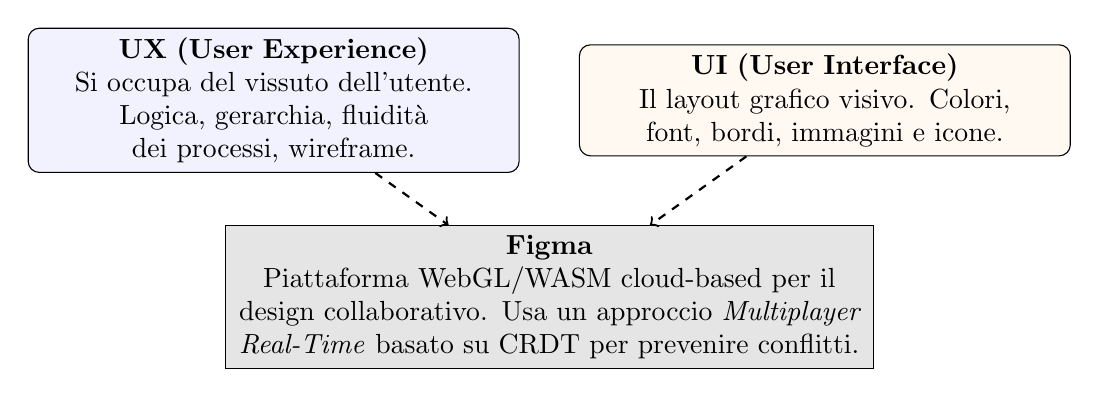
\begin{tikzpicture}
        % UI vs UX Box
        \node[draw, rounded corners, fill=blue!5, text width=6cm, align=center] (UX) at (-3.5,0) {
            \textbf{UX (User Experience)}\\
            Si occupa del vissuto dell'utente.
            Logica, gerarchia, fluidità dei processi, wireframe.
        };

        \node[draw, rounded corners, fill=orange!5, text width=6cm, align=center] (UI) at (3.5,0) {
            \textbf{UI (User Interface)}\\
            Il layout grafico visivo.
            Colori, font, bordi, immagini e icone.
        };

        \node[draw, fill=gray!20, text width=8cm, align=center] (Figma) at (0,-2.5) {
            \textbf{Figma}\\
            Piattaforma WebGL/WASM cloud-based per il design collaborativo.
            Usa un approccio \textit{Multiplayer Real-Time} basato su CRDT per prevenire conflitti.
        };

        \draw[->, thick, dashed] (UX) -- (Figma);
        \draw[->, thick, dashed] (UI) -- (Figma);
    \end{tikzpicture}
\end{center}